% Generated from the public primitive catalog. Original Atlas drawing; Apache-2.0.
% Target: chacha20-poly1305-ietf; view: detail
\documentclass[border=9pt]{standalone}
% Original Atlas figure theme. Apache-2.0; see the repository LICENSE.
\usepackage[T1]{fontenc}
\usepackage{lmodern}
\usepackage{amsmath,amssymb}
\usepackage{tikz}
\usetikzlibrary{arrows.meta,positioning,calc,fit,backgrounds,decorations.pathreplacing,matrix}
\definecolor{atlasInk}{HTML}{172235}
\definecolor{atlasTeal}{HTML}{0D7B7D}
\definecolor{atlasMuted}{HTML}{637278}
\definecolor{atlasFill}{HTML}{EAF4F2}
\definecolor{atlasLine}{HTML}{B6C8C7}
\tikzset{
  every picture/.style={line width=.65pt,draw=atlasInk,>=Latex},
  every node/.style={text=atlasInk,font=\sffamily\small},
  box/.style={draw,rounded corners=1.5pt,minimum height=.9cm,minimum width=1.6cm,align=center,inner sep=6pt,fill=white},
  accent/.style={box,draw=atlasTeal,fill=atlasFill},
  wire/.style={->,line width=.7pt},
  keywire/.style={wire,draw=atlasTeal,dashed},
  xor/.style={draw,circle,fill=white,inner sep=0pt,minimum size=.38cm},
  add/.style={draw,rectangle,fill=white,inner sep=0pt,minimum size=.38cm},
  note/.style={font=\sffamily\scriptsize,text=atlasMuted,align=center},
  phase/.style={font=\sffamily\small\bfseries,text=atlasTeal},
  group/.style={draw=atlasLine,dashed,rounded corners=2pt,inner sep=8pt}
}
\newcommand{\rotl}{\mathbin{\lll}}
\newcommand{\rotr}{\mathbin{\ggg}}
\newcommand{\kx}{\operatorname{Keccak}\!\text{-}\!f[1600]}

\newcommand{\AtlasKeyBits}{256}
\newcommand{\AtlasKeyWords}{8}
\newcommand{\AtlasRounds}{N_r}
\newcommand{\AtlasPriorRounds}{N_r-1}
\newcommand{\AtlasRoundKeys}{N_r+1}
\newcommand{\AtlasDoubleRounds}{N_r/2}
\newcommand{\AtlasSixRoundGroups}{N_r/6}
\newcommand{\AtlasFLGroups}{N_r/6-1}
\newcommand{\AtlasRoundStart}{24-n}
\newcommand{\AtlasBlockBits}{b}
\newcommand{\AtlasOutputBits}{d}
\newcommand{\AtlasStateBits}{8w}
\newcommand{\AtlasNonceBits}{96}
\newcommand{\AtlasCounterBits}{q}
\newcommand{\AtlasStreamBlockBits}{b}
\newcommand{\AtlasRate}{r}
\newcommand{\AtlasCapacity}{c}
\newcommand{\AtlasSteps}{N}
\newcommand{\AtlasLastStep}{N-1}
\newcommand{\AtlasWordBits}{w}
\newcommand{\AtlasHashWords}{h}
\newcommand{\AtlasFeedForward}{\boxplus}
\newcommand{\AtlasByteOrder}{big-endian}
\newcommand{\AtlasDomain}{01}
\newif\ifAtlasXof
\AtlasXoffalse
\begin{document}
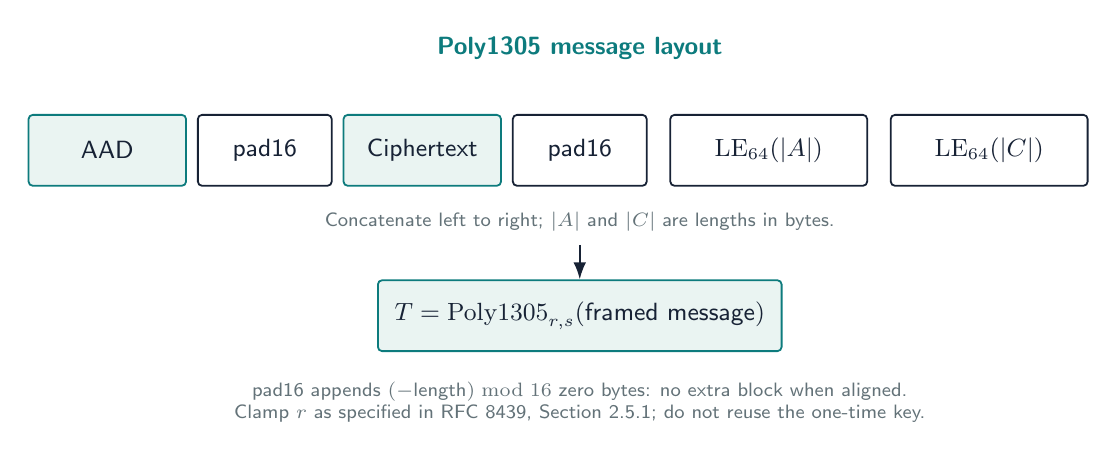
\begin{tikzpicture}
  \node[phase] at (6,2) {Poly1305 message layout};
  \node[accent,minimum width=2cm] (a) at (0, .7) {AAD};
  \node[box,minimum width=1.7cm] (pa) at (2, .7) {pad16};
  \node[accent,minimum width=2cm] (c) at (4, .7) {Ciphertext};
  \node[box,minimum width=1.7cm] (pc) at (6, .7) {pad16};
  \node[box,minimum width=2.5cm] (la) at (8.4, .7) {$\operatorname{LE}_{64}(|A|)$};
  \node[box,minimum width=2.5cm] (lc) at (11.2, .7) {$\operatorname{LE}_{64}(|C|)$};
  \node[note] at (6,-.2) {Concatenate left to right; $|A|$ and $|C|$ are lengths in bytes.};
  \node[accent,minimum width=5cm] (mac) at (6,-1.4) {$T=\operatorname{Poly1305}_{r,s}(\text{framed message})$};
  \draw[wire] (6,-.5) -- (mac);
  \node[note] at (6,-2.5) {pad16 appends $(-\text{length})\bmod16$ zero bytes: no extra block when aligned.\\Clamp $r$ as specified in RFC 8439, Section 2.5.1; do not reuse the one-time key.};
\end{tikzpicture}

\end{document}
